
%(BEGIN_QUESTION)
% Copyright 2007, Tony R. Kuphaldt, released under the Creative Commons Attribution License (v 1.0)
% This means you may do almost anything with this work of mine, so long as you give me proper credit

Single-tube manometers (called {\it piezometers}, which literally means ``pressure meters'') installed on a level venturi tube clearly show the difference in pressure at different points within the tube.  These pressure differences, of course, are due to the exchange of energy between potential and kinetic forms:

$$\includegraphics[width=15.5cm]{i02980x01.eps}$$

Note that the following form of Bernoulli's equation is used to describe pressure and height in the diagram, for the purpose of expressing all terms as vertical distances (in units of feet).  This is why pressure is shown as $P / \gamma$ instead of just $P$:

$$z_1 + {v_1^2 \over {2 g}} + {P_1 \over \gamma} = z_2 + {v_2^2 \over {2 g}} + {P_2 \over \gamma}$$

If we install three more piezometer tubes -- this time with their tube ends facing the direction of oncoming liquid flow (called {\it Pitot tubes}) -- we see something quite interesting: the heights of liquid in all the new tubes are equal.

$$\includegraphics[width=15.5cm]{i02980x02.eps}$$

What accounts for the difference in height between liquid columns in the three sets of piezometers?  How come the Pitot tube piezometers all register the same height?  What is the significance of the line where all the Pitot tube piezometer liquid levels are equal?

\underbar{file i02980}
%(END_QUESTION)





%(BEGIN_ANSWER)

The difference in height is due to the ``velocity head'' at each point:

$$\includegraphics[width=15.5cm]{i02980x03.eps}$$

The line where all the Pitot tube piezometers match is sometimes called the {\it energy line} of the system.

\vskip 10pt

Follow-up question: in a realistic piping system, this energy line has a downward slope.  Explain why:

$$\includegraphics[width=15.5cm]{i02980x04.eps}$$

%(END_ANSWER)





%(BEGIN_NOTES)

The answer to the follow-up question, of course, is energy loss due to friction.  This loss occurs in the ``pressure head'' terms ($P / \gamma$) of Bernoulli's equation, since neither the liquid heights nor the liquid velocities are different in similar-sized sections of the pipe.  Note that the continuity equation ensures velocities must be equal in areas of equal cross-sectional area for a liquid flow stream ($\rho_1 A_1 v_1 = \rho_2 A_2 v_2$).


%INDEX% Measurement, flow: Pitot tube
%INDEX% Measurement, pressure: piezometer
%INDEX% Physics, dynamic fluids: Bernoulli's equation

%(END_NOTES)


